\pagenumbering{arabic}
\setcounter{chapter}{0}
\chapter{Vehicle Models}
\section{Unicycle model}

\begin{align}
\dot{x} &= u_s\cos{\theta}\\
\dot{y} &= u_s\sin{\theta}\\
\dot{\theta} &= u_\omega
\end{align}
\subsection{Reed Shepp's Car}
A Unicycle model can simulate a Reed-Shepp's car with 
\begin{itemize}
    \item $u_s \in \{-1, 0, 1\}$
    \item Transformation $u_{\omega}=\frac{\tan{\delta}}{L}$
    \item restricting $\delta$ to $[-\delta_{max}, \delta_{max}]$ where $\delta$ represent the steering angle and $\frac{L}{\tan\delta}$ represents the turning radius. $L$ is the wheel-base.
\end{itemize} 
\subsection{Dubin's Car}
Dubin's car is a simplification of Reed-Shepp's car  with $u_s \in \{0, 1\}$ 

\shabox{A unicycle model can simulate a Reed-Shepp's car, Dubin's car and the Single track rear wheel model below when steering is the control input without considering the steering rate. It can also simulate tricycle and differential drive robot. The details are not discussed here explicitly}

\section{Single Track Rear Wheel Model}
For a front-wheel driven vehicle with no slip
\begin{align}
\dot{x} &= u_s\cos{\theta} \\
\dot{y} & = u_s\sin{\theta} \\
\dot{\theta} & = u_s \frac{\tan{\delta_r}}{L} \\
\dot{\delta_r} &= u_\delta
\end{align}
where $L$ is the wheel base and the state represents the rear-wheel, $\delta_r$ represents the steering angle at the rear wheels and $u_s$ is the speed of the rear-wheel

The Single track rear wheel model can be further expanded out to include acceleration  as
\begin{align}
\dot{x} &= u_s\cos{\theta} \\
\dot{y} & = u_s\sin{\theta} \\
\dot{\theta} & = u_s \tan{\delta_r}/L \\
\dot{u_s} &= u_a \text{(or other first order approximations/reduced order models)} \\
\dot{\delta_r} &= u_\delta
\end{align}
the control input is $u=[u_a  u_\delta]^{'}$
If curvature is the input to the system, the model can be rewritten as
\begin{align}
\dot{x} &= u_s\cos{\theta} \\
\dot{y} & = u_s\sin{\theta} \\
\dot{\theta} & = u_s \kappa \\
\dot{u_s} &= u_a \text{(or other first order approximations/reduced order models)}
\end{align}
where $\kappa$ indicates the curvature value
\section{Single Track Front Wheel Model}
For a front-wheel driven vehicle with no side slip
\begin{align}
\dot{x} &= u_s\cos({\theta + \delta}) \\
\dot{y} & = u_s\sin({\theta + \delta}) \\
\dot{\theta} & = u_s \frac{\sin{\delta}}{L} \\
\dot{\delta_f} &= u_\delta
\end{align}
where $\delta_f$ represents the steering angle at the front wheels wheels.
This model can be augmented with acceleration commands instead of speed similar to the equations presented in the rear wheel models.

Furthermore, the models can be rewritten using curvature instead of steering angles or steering rate. Additionally, there are limits on speed, acceleration, steering, steering rate and curvature.
\section{Model with Slip}
Assuming the vehicle can be steered with both front and rear wheels, the model equations with slip $\beta$ are
\begin{align}
\dot{x} &= u_s\cos(\theta+\beta) \\
\dot{y} &= u_s\sin(\theta+\beta) \\
\dot{\theta} &= u_s\frac{\cos{\beta}}{l_f+l_r}(\tan\delta_f - \tan\delta_r) \\
\dot{u_s} &= u_a \\
\beta & = \arctan(\frac{l_f\tan\delta_r+l_r\tan\delta_f}{l_f+l_r})
\end{align}
where $\beta$ denotes vehicle slip angle, $l_f$ is the distance of the front wheels to the center of mass, $l_r$ is the distance of the rear wheels to the center of mass, $\delta_f$ is the front wheel steer and $\delta_r$ is the rear wheel steer
\begin{figure}[!ht]
\centering
 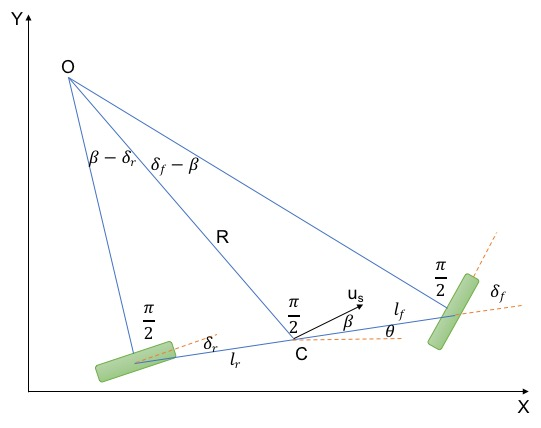
\includegraphics[width=0.8\textwidth]{slip_kinematic_model.jpg}   
\caption{Kinematic vehicle model with Slip and front and rear wheel steer. O is the instantaneous center of rotation} \label{fig:slip_kin_model}
\end{figure}
\subsection{Derivation}
From left triangle, applying the sine rule
\begin{align}
    \frac{\sin(\frac{\pi}{2}+\delta_r)}{R} &= \frac{sin(\beta-\delta_r)}{l_r} \\
    \implies \frac{l_r}{R} &= \sin\beta - \tan\delta_r\cos\beta \label{eq:rear_slip_beta}
\end{align}
From the triangle on the right, applying the sine rule
\begin{align}
    \frac{\sin(\frac{\pi}{2}-\delta_f)}{R} &= \frac{sin(\delta_f - \beta)}{l_f} \\
    \implies \frac{l_f}{R} &= \tan\delta_f\cos\beta - \sin\beta  \label{eq:front_slip_beta}
\end{align}
Divide equations (\ref{eq:rear_slip_beta}) and (\ref{eq:front_slip_beta}), we have
\begin{align}
    \frac{l_r}{l_f}&=\frac{\sin\beta - \tan\delta_r\cos\beta}{\tan\delta_f\cos\beta - \sin\beta} \\
    \implies \frac{l_r}{l_f}&=\frac{\tan\beta-\tan\delta_r}{\tan\delta_f - \tan\beta} \\
    \implies \tan\beta &= \frac{l_r\tan\delta_f + l_f\tan\delta_r}{l_f+l_r}
\end{align}
Now we know that $\dot{\theta}=\frac{u_s}{R}$. To derive $R$, we use (\ref{eq:rear_slip_beta}). Substituting $\tan\beta$ derived above into \ref{eq:rear_slip_beta}, we have
\begin{align}
    \frac{l_r}{R} &= \cos\beta(\tan\beta - \tan\delta_r) \\
    \implies \frac{l_r}{R} &= \cos\beta(\frac{l_r\tan\delta_f + l_f\tan\delta_r}{l_f+l_r} - \tan\delta_r) \\
    \implies \frac{l_r}{R} &= \frac{\cos\beta}{l_f+l_r}(l_r\tan\delta_f - l_r\tan\delta_r) \\
    \implies \frac{1}{R} &= \cos\beta\frac{\tan\delta_f - \tan\delta_r}{l_f+l_r} \\
    \implies \dot{\theta}&=\frac{u_s}{R}= u_s\cos\beta\frac{\tan\delta_f - \tan\delta_r}{l_f+l_r}
\end{align}
As far the equations for $x$ and $y$ go, it is straightforward to see that
\begin{align}
    \dot{x}&=u_s\cos(\theta+\beta) \\
    \dot{y}&=u_s\sin(\theta+\beta) \\
\end{align}

\section{Dynamic Lateral and Longitudinal Model} 
\subsection{Lateral Dynamics}
The lateral dynamics is given by
\begin{align}\label{eq:lat_dynamics}
    ma_y &=m\Ddot{y} + u_{sx}\dot{\theta} = F_{yf} + F_{yr} + F_{bank} \\
    I_z\Ddot{\theta} &= l_fF_{yf}-l_rF_{yr}
\end{align}
where $F_{yf}$ and $F_{yr}$ denote the lateral tire forces at the front and rear wheels, $m$ is the mass of the vehicle, $u_sx$ is the longitudinal speed of the vehicle at CG. 

\shabox{Slip is the difference in angle between velocity vector at the wheel and the steering angle}

For small slip angles (i.e. lower speeds <~35-40 mph typically for nominal friction conditions i.e no sleet, water, ice etc), they are approximated by (for front wheel drive) a linearly as.
\begin{align}
    F_{yf} &= 2C_{\alpha f}(\delta-\theta_{vf}) \\
    F_{yr} &= 2C_{\alpha r}(-\theta_{vr})
\end{align}
where $C_{\alpha f}$ and $C_{\alpha r}$ represent the cornering stiffness of each of the front and rear wheels respectively.
$F_{bank} = mg\sin\phi$, where $\phi$ is the bank angle, $g$ is the acceleration due to gravity
The velocity vector at the wheels are given by
\begin{align}
    \tan{\theta_{vf}} &= \frac{u_sy+l_f\dot{\theta}}{u_sx} \\
    \tan{\theta_{vr}} &= \frac{u_sy-l_r\dot{\theta}}{u_sx}
\end{align}
Using small angle approximations, the above equations can be further reduced to 
\begin{align}
    \theta_{vf} &= \frac{\dot{y}+l_f\dot{\theta}}{u_sx} \\
    \theta_{vr} &= \frac{\dot{y}-l_r\dot{\theta}}{u_sx}
\end{align}
\subsection{Longitudinal Dynamics}
\begin{figure}
    \centering
    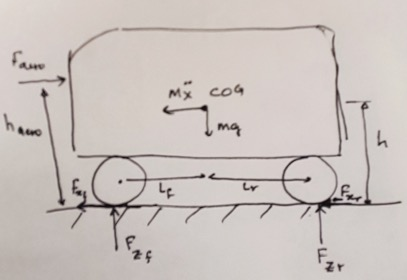
\includegraphics{veh_long_dyn.jpg}
    \caption{Longitudinal forces on the vehicle}
    \label{fig:veh_long_dyn}
\end{figure}
Ignoring the pitch of the vehicle i.e. assuming flat surface, the longitudinal dynamics is given by
\begin{align}
    m\Ddot{x}&=F_{xf} + F_{xr} - F_{aero} - R_{xf} - R_{xr}
\end{align}
where $F_{xf}$ and $F_{xr}$ denote the longitudinal forces at the front and rear wheels respectively, $F_{aero}$ denotes aerodynamics drag force, $R_{xf}$ and $R_{xr}$ denote rolling resistance at the front and rear wheels
Aerodynamic drag force is given by
\begin{align}
    F_{aero} &= \frac{1}{2}\rho C_dA_F(V_x+V_{wind})^2
\end{align}
where $\rho$ is the density of air, $C_d$ is the aerodynamic drag coefficient, $V_x$ is the longitudinal speed of the vehicle, $V_wind$ is the wind velocity and $A_F$ is the frontal area of the vehicle.
The longitudinal tire forces are a function of slip, normal load on the tire and the friction coefficient.
The longitudinal slip ratio is defined as
\begin{align}
    \sigma_{long} &= \frac{r_{eff}\omega_{wheel}-V_x}{V_x} \textsc{braking} \\
    \sigma_{long} &= \frac{r_{eff}\omega_{wheel}-V_x}{r_{eff}\omega_{wheel}} \textsc{acceleration} 
\end{align}
where $\omega_{wheel}$ is the rotational speed of the wheel and $r_{eff}$ is the effective tire radius.
When the slip is small, the longitudinal forces are given by
\begin{align*}
    F_{xf} &= C_{\sigma f}\sigma_{xf} \\
    F_{xr} &= C_{\sigma r}\sigma_{xr}
\end{align*}
where $C_{\sigma f}$ and $C_{\sigma r}$ represent longitudinal stiffness at front and rear wheels.

The rolling resistance $R_{xf}$ and $R_{xr}$ are approximated using the coefficient of friction and the normal loading force at the front wheel $F_{zf}$ and rear wheel $F_{zr}$ as
$$R_{xf} + R_{xr} = f (F_{zf} + F_{zr})$$.
When the vehicle is travelling along a surface with no gradient, $F_{zf}$ and $F_{zr}$ are in turn calculated by taking moments about the contact points of the front and rear wheels as 
(see Figure~\ref{fig:veh_long_dyn}) 
\begin{align}
    F_{zf}(l_f+l_r) + F_{aero}h_{aero} -m\Ddot{x}h - mgl_r &= 0 \\
    F_{zr}(l_f+l_r) - F_{aero}h_{aero} +m\Ddot{x}h - mgl_f &= 0 
\end{align}
The above equations can be straightforwardly extended to the case when the vehicle is pitching while maintaining contact with the ground i.e when the vehicle is moving on an inclined surface. (the terms that correspond $mg$ will have additional component along and perpendicular to the surface)
\subsection{Error models}
\subsubsection{With respect to the road}
Let's say the objective is to follow the center line of the road. At any given point let $\theta_{des}$ be the headong of the centerline. The lateral acceleration desisred at this point would be $V_x\theta_{des}$. The lateral acceleration of the vehicle in the inertail coordinates is $a_y = \Ddot{y} + V_x\theta$ where $V_x$ is the longitudinal speed of the vehicle in the body frame and $\theta$ is the heading of the vehicle. The error equations under the assumption of constant longitudinal speed can be written as
\begin{align}
    \dot{e_1} &= \Ddot{y} + V_x(\dot{\theta} - \dot{\theta_{des}}) \\
    \dot{e_2} & = \dot{\theta} - \dot{\theta_{des}}
\end{align}
where $e_1 = \dot{y} + V_x(\theta - \theta_{des})$ and $e_2 = \theta - \theta_{des}$
The error dynamics can now be obtained using~(\ref{eq:lat_dynamics}). The model now can be used for developing steering control law the objective of which would be to stabilize the above system.
\section{Linearization}
Let's say a dynamic system is defined by
\begin{align}
    \dot{x} &= f(x, u)
\end{align}
where $x$ is the state and $u$ is the control input
The linearized system is given by
\begin{align}
    \dot{\delta x} = \frac{\partial f}{\partial x} \delta x + \frac{\partial f}{\partial u} \delta u + H.O.T
\end{align}
H.O.T (Higher order terms) are generally neglected under the assumption that $\delta x$ and $\delta u$ are small. Linearization is generally used for stability analysis and for designing controllers for reference and trajectory tracking (example LQR, MPC etc) 

First define $\delta x = x - x^{*}$ and $\delta u = u - u^{*}$ where $x^*$ and $u^*$ represent the state and control inputs at equilibrium  or define the operating points i.e. trim conditions.
The derivation proceeds as follows
\begin{align}
    \dot{\delta x} &= \dot{x} - \dot{x^*} \\
    \implies \dot{\delta x} &= f(x, u) - f(x^*, u^*) \\
    \implies \dot{\delta x} &= f(x^* + \delta x, u^* + \delta u)- f(x^*, u^*)
\end{align}
Taylor series expansion can now be used to derive the equations above. 

H.0.T some times are used to a second degree in methods like DDP (Differential Dynamic Programming).We will discuss more about this in another chapter. 

\subsubsection{Example}
Let's take the example of the simplified single track rear wheel model. The equations for the simple car model are given by
\begin{align*}
    \dot{x} &= u_1\cos{\theta} \\
    \dot{y} &= u_1\sin{\theta} \\
    \dot{\theta} &= u_1\frac{\tan u_2}{L}
\end{align*}
where $u_1$ is the speed control input and $u_2$ is the steering control input with $L$ as the wheel base.

Using the derivation, let's linearize the system about the state $[{}0,{}0, {}pi/4{}]$ and control $[{}1, {}0{}]$
\begin{align}
    \dot{\delta x} &= 0 \times \delta x + 0 \times \delta y - (u_1=1)\times\sin(\theta = \frac{pi}{4}) \times \delta \theta + \delta u_1 \\
    \dot{\delta y} &= 0 \times \delta x + 0 \times \delta y + (u_1=1)\times\cos(\theta = \frac{pi}{4}) \times \delta \theta + \delta u_1 \\
    \dot{\delta \theta} &=  0 \times \delta x + 0 \times \delta y + 0\times\delta \theta + \frac{\tan (u_2=0)}{L} \times \delta u_1+ (u_1=1)\times\frac{\sec^2 (u_2=\frac{pi}{4})}{L}\times\delta u_2 
\end{align}
In matrix form it can be represented as
\begin{align}
    \begin{bmatrix}
          \dot{\delta x}\\
          \dot{\delta y} \\
         \dot {\delta \theta}
    \end{bmatrix} & =  \begin{bmatrix}
    0 & 0 & -\frac{1}{\sqrt{2}} \\
    0 & 0 & \frac{1}{\sqrt{2}} \\
    0 & 0 & 0
    \end{bmatrix}
    \begin{bmatrix}
          \delta x\\
          \delta y \\
         \delta \theta
    \end{bmatrix} + \begin{bmatrix}1 & 0 \\ 1 & 0 \\ 0 & \frac{2}{L}\end{bmatrix}\begin{bmatrix}\delta u_1 \\ \delta u_2\end{bmatrix}
\end{align}

\shabox{The controllability rank condition is not met by the linearized system. However the original nonlinear model i.e. the simple car model is Small Time Locally Controllable (STLC) - we will talk about this later}